\documentclass{IEEEtran}

\usepackage[utf8]{inputenc}
\usepackage[top=2cm,left=2cm,right=2cm]{geometry}
\usepackage{graphicx}
\usepackage{caption}
\usepackage{subcaption}

\usepackage{fancyhdr}
\pagestyle{fancy}
\fancyhf{}
\lhead{Landon Buell}
\rhead{B.S. Physics Thesis}
\cfoot{\thepage}

\title{Approximate Computation Image Classification}
\author{Landon Buell}
\date{August 2022}

\begin{document}

\maketitle

\begin{abstract}

Computer vision is a prominent and ever-growing subfield of Artificial Intelligence born out of digital image processing.  As increasingly powerful processors and more disk space becomes available to the commercial, academic, and consumer worlds, the size of image datasets has also increased as well. Storing large masses of input data is a common problem in the world of AI and is routinely revisited. Similarly, most computer vision models are architected to accept images that all have a consistent size within a dataset. These problems combined highlight the need for a more efficient method of storing volumes of image data, without compromising the performance of the models that will process them. In this experiment, we explore a possible solution to this issue where we down-sample images to store them at a fraction of the disk size, and then use various interpolation techniques to rebuild them up to the original size. We explore how the down-sized, then up-scaled images compare a baseline, and then offer a discussion for the viability of this as a long term solution. 

\end{abstract}

% ================================================================
\section{Introduction}

Deep image classification is type of Computer Vision which employs deep neural networks to organize images into categories based on their contents of properties \cite{Goodfellow,Loy}. This practice can be seen widely in the modern world in instances such as facial recognition, parsing of handwriting, and image database organization. Note that in image classification inputs are assigned a label based on the aggregate contents of the image, whereas in object detection or segmentation, is attempting to isolate a set of pixels that correspond to an object of interest. For this study, focus solely on image classification.

In their raw format, modern digital images are typically organized as 2-dimensional arrays of gray-scale images, or 3-dimensional arrays for color images. This format allows them to very informationally dense, making them highly effective in classification, but comes at the cost of being large to store or computationally taxing to process \cite{Goodfellow}. A single 1080 x 1920 RGB image contains more than 6.2 million pixels, each stored as a byte. When processed by a neural network, each byte is upcast to a single-precision float which brings that same object up to more than 24.8 million bytes. This problem becomes even more pronounced when considering 4K resolution images which in their raw form are 3840 x 2160 x 3 pixels, or around 24.8 million bytes, and almost 100 million bytes when upcast to single precision. While modern compression formats such as JPEG or PNG can reduce this size on disk by nearly an order of magnitude, storing massive quantities of samples can still be taxing. 

% ================================================================
\section{Dataset}

Since the 1980's the United State Postal Service, (USPS) has been using image artificial intelligence, and image classification to identify hand-written characters at a rate far fast than humans ever could. Over many years, some of these characters have been organized into the \textit{MNIST-784} data set. In this collection, there are $70,000$ uniuque samples, each containing a centered, $28$ x $28$ gray-scale image of a hand-written digit, $0$ through $9$ with an appropriate label. The MNIST-784 data set was accessed through the \textit{sklearn} python library \cite{Sklearn}.

\begin{figure}[h]
    \centering
    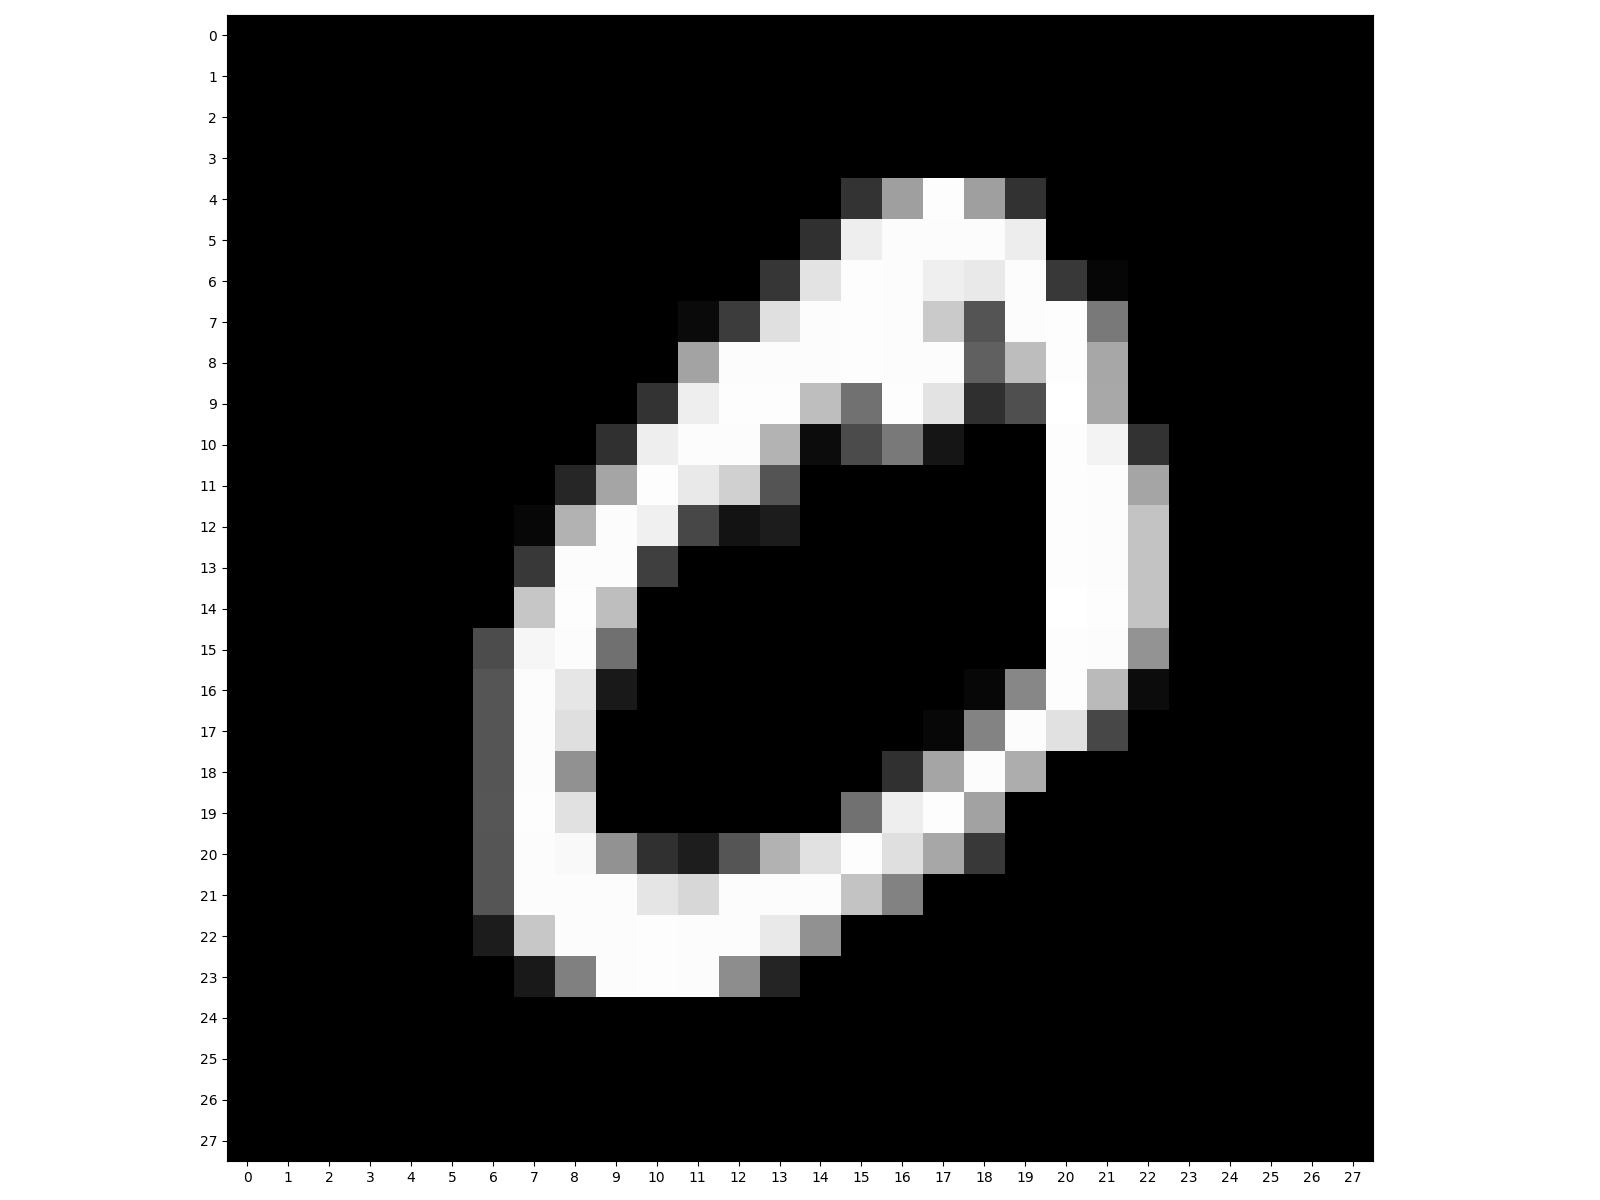
\includegraphics[scale=0.1]{fig/baseline1.png}\hfill
    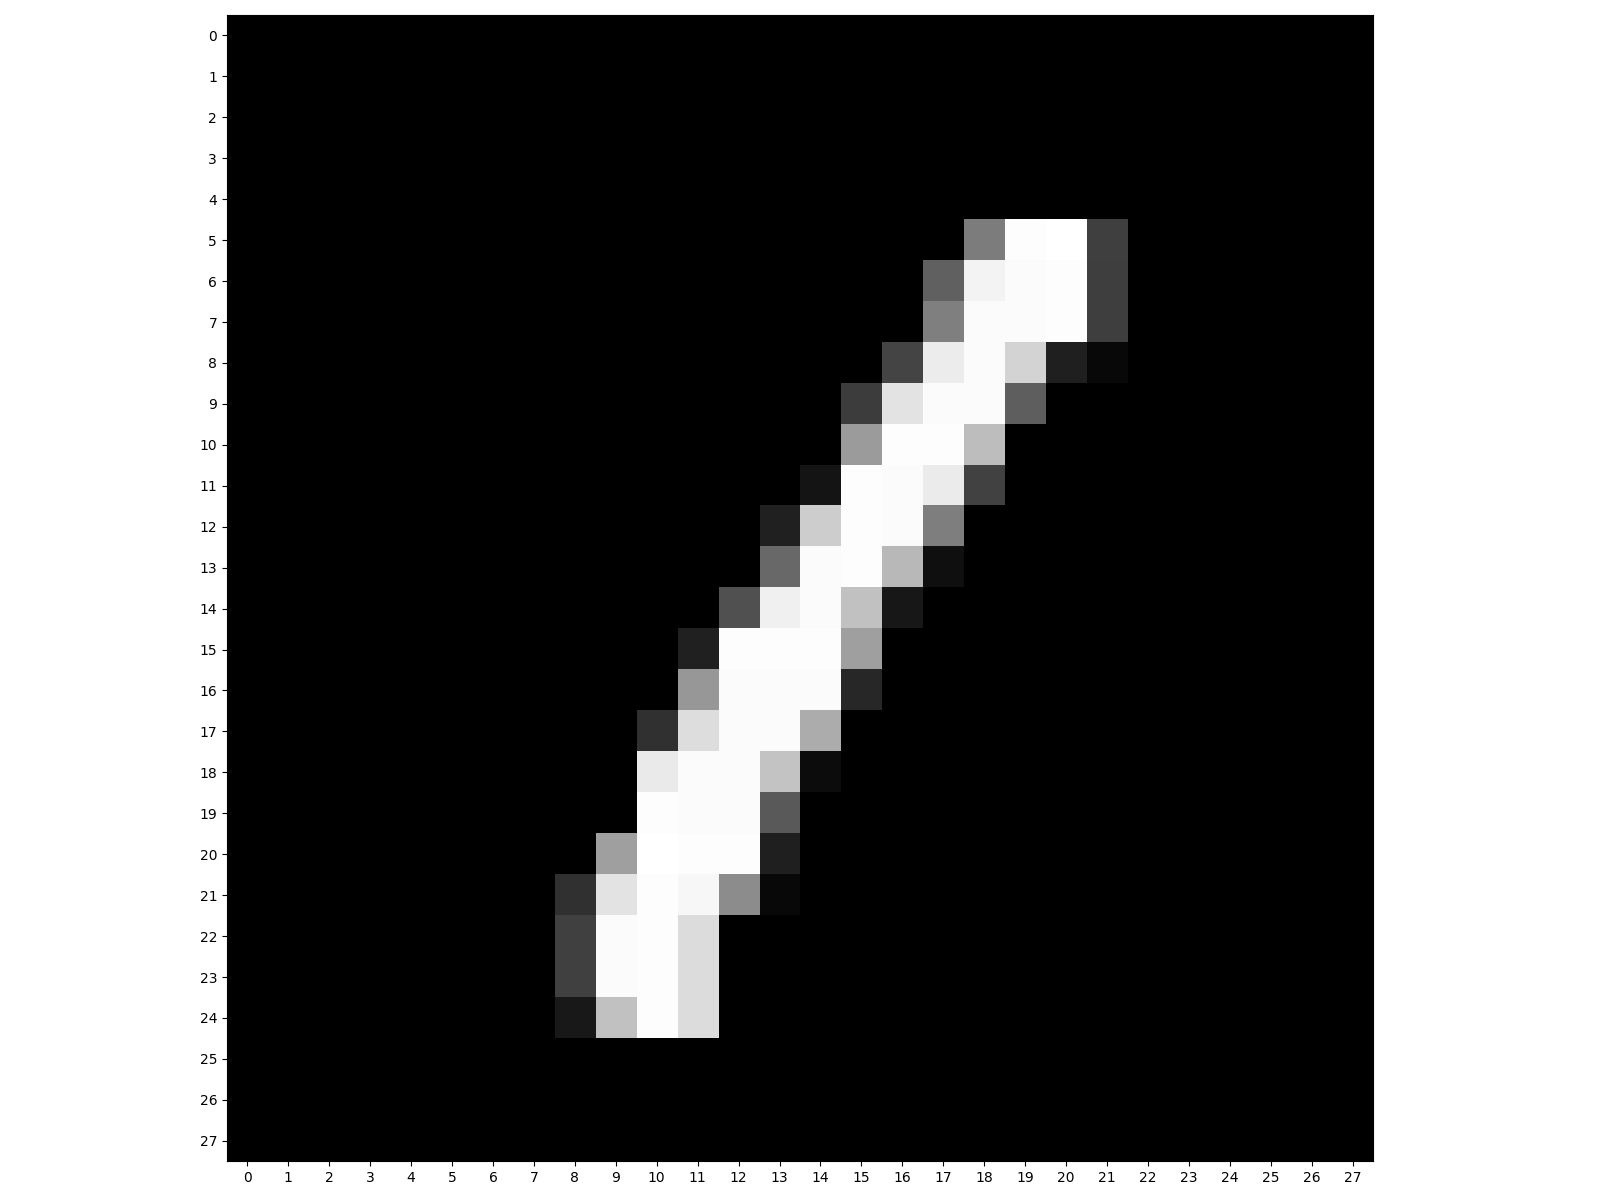
\includegraphics[scale=0.1]{fig/baseline3.png}
    \caption{Example images from the MNIST-784 database. Each image here is stored as a grid of bytes, plotted in 28 x 28 gray-scale. Figures generated with \textit{matplotlib} and \textit{numpy} python libraries. \cite{Matplotlib,Numpy}}
    \label{fig:Mnist784}
\end{figure}

Before presented to the neural network, the data set upcast from bytes to single-precision floating-point numbers and is subject to a \textit{standard-scaling} step. In standard scaling, the data set is transformed such that each across all samples, any single feature (pixel) has zero mean and unit variance. This has the effect of "centering" the data in feature space, and reducing the magnitude of any major outlying values. This prevents any machine learning model from inadvertently biasing certain pixels over other and generally yields an overall better fit \cite{Geron,Loy,James,Sklearn}.

% ================================================================
\section{Linear Interpolation}

Interpolate is a type of mathematical estimation that involves determining new data samples based on a set of existing samples. Note that in this experiment, interpolation should not be considered to be machine learning, but is rather a fixed procedure. We use 2D interpolation as a preprocessing step to modify input images, which are then fed to a neural network. Since images are simply 2D or 3D arrays of pixels, we can leverage python's \textit{scipy} library \cite{Scipy} to aid with the interpolating of images as if they represent the output of an arbitrary function of two input variables, one for each axis.

For any image that has been down-sized to $q'$ x $q'$, we can use interpolation to up-sample it back to $q$ x $q$. \textbf{FINISH THIS}

% ================================================================
\section{Deep Neural Network Architecture}

At a high level, a neural network can be treated as a function $F$ that maps inputs $x$ called features, to outputs $y^*$ called predictions, using a set of parameters $\Theta$. 

\begin{equation}
    \label{NeuralNetworkFunction}
    F : x^{(0)},\Theta \rightarrow y^*
\end{equation}

Buried within this function $F$, is a set of $L$ smaller composite functions called \textit{layers}. The values computed and store within each layer function are refereed to as the \textit{activations} of that layer. Each layer function $f^{(l)}$ takes the previous layer's activations $x^{(l-1)}$, and transforms them into $x^{(l)}$ using parameters $\Theta^{(l)}$ \cite{Goodfellow}. We denote any layer:
\begin{equation}
    \label{LayerFunction}
    f^{(l)} : x^{(l-1)}, \Theta^{(l)} \rightarrow x^{(l)}
\end{equation}
Note the activations of the final layer, $x^{(L-1)}$ are the outputs of the model, $y^*$ as shown in Eq. (\ref{NeuralNetworkFunction}). We use the Python library \textit{tensorflow 2} to contruct, train, and evaluate neural network models \cite{Tensorflow}.

\subsection{The Convolutional Neural Network}

TODO - THIS!


\subsection{Model Configuration}

TODO - THIS!

\subsection{Objective Function} 
For any sample $x_{i}$, there is an associated ground truth $y_i$ called a label. However, when input $x_i$ is provided to the neural network, it returns an output $y_i^*$. To compare the the output to the label, we introduce an object function, $J(y,y^*)$ which returns a scalar value proportional to their difference \cite{James}. For this $k$-class classification experiment, we choose to use \textit{categorical crossentropy} objective as shown in Eq. \ref{CategoricalCrossentropy} (CXE) \cite{Geron,Virtanen,Tensorflow}. This objective assumes both the outputs and labels to $1$ x $k$ vectors, with $L-1$ norms of 1.
\begin{equation}
    \label{CategoricalCrossentropy}
    {CXE}[y,y^*] = - \sum_{i=0}^{k-1} y[i]\ln(y^*[i])
\end{equation}
For trained deep neural network we expect a consistently low objective value across a collection of inputs, meaning that the model can correctly match inputs to intended outputs. Therefore the process of training a model is optimizing the elements in $\Theta$ to minimize the value of the objective function, in the assumption that doing so will also improve the performance of the model \cite{Goodfellow}.

\subsection{Optimization Algorithm}  
An optimization algorithm is the procedure used by a machine learning model to train itself. Due to the composite nature of deep neural networks, an exact expression to optimize may be impractical to generate and solve with traditional symbolic mathematics, so we typically resort to iterative, gradient-based techniques \cite{Goodfellow, Geron, Loy}. These techniques involve repeatedly: (1) passing a batch of labeled samples through an untrained model, and then computing the objective value (2) Computing the gradient of the objective function with respected to all elements in $\Theta$, and (3) Scaling each parameter in $\Theta$ proportionally to the object value and the negative gradient for that parameter. This process is called \textit{stochastic gradient descent} (SGD). Executing this multiple times over a collection of samples gradually drives the objective function value down, indicating that the model is learning how to correctly map inputs $x$ to outputs $y$.

SGD optimization by itself can often be unstable, and prone to numerical errors. To combat this, we employ an \textit{Adaptive Moments} optimizer, also called ADAM. ADAM uses an adaptive learning rate and a built-in momentum parameter to execute a far more aggressive and robust optimization procedure \cite{Goodfellow}. As the optimizer proceeds with a set of training data, the effects of past iterations may snowball, and allow the process to overcome small discontinuities that may arise in the solution space.

\subsection{Metric Functions} -
To quantify the performance of a classification model, we choose numerous metric functions that inform us as to how a model is learning. \\
\textbf{ (1) Objective Value - } Provides a rough indication of how well the model is is trained. A consistently low objective value means that the model has learned a set of parameters in $\Theta$ that allow is to correctly match inputs to intended outputs. The scalar value itself does not provide much information on the intricacies of how the model is performing. \\
\textbf{(2) Precision - } determines what fraction of chosen items are relevant to the problem. It is bound on the interval $[0,1]$ with a higher score as more favorable. If a model reports a precision score of identically $1$, then no false-positives were chosen. \\
\textbf{(3) Recall - } determines what fraction of relevant items to the problem were chosen. It is bound on the interval $[0,1]$ which a higher score as more favorable. If a model reports a recall score of identically $1$, then no false-negatives were chosen. \\
\textbf{(4) F1-Score - } is the harmonic mean of precision and recall scores. The higher both scores, the higher the resulting F1-score is. 

% ================================================================
\section{Experiment Methodology}
For the baseline experiment and each successive case-study, we follow a similarly structured procedure. In each case study, every raw 28 x 28 gray-scale image is down-sampled to a smaller size to simulate how that image could be stored on disk. We then use a 2D linear spline interpolation to up-sample that image back to the original 28 x 28 pixel size. The result is a collection of perturbed images that are used to train and test a collection of neural network models. For each case study, we indicate the size of the "compressed" image and the number of resulting pixels compared to the full size.

For every case, including the baseline, we use 80\% of the samples for training a model, and 20\% of the samples to test it's performance. In all cases, any preprocessing has been applied to every sample in the data set before the train-test process occurs. This means that a model that is trained on down-sampled and then interpolated up is also evaluated on samples that have had the same procedure applied.  For the baseline and each of the case studies, we repeat a nearly identical experiment $10$ times for thoroughness. In each iteration, we update a "random state" value when generating a new model, which changes the initialize state of the generated parameters in the $\Theta$ object. We also use the changing random state to change how samples are shuffled in the train-test split procedure.

\subsection{Baseline}
For the baseline, no additional preprocessing was applied to each sample. The data set was scaled and then provided to a neural network as-is. 

\subsection{Case Study 1}
Each input sample is subject to a 2D average pooling filter which uses a 2 x 2 window, with a 1 x 1 step size, which brings the image from 28 x 28 down to 27 x 27. In this format each image is 729 pixels, or $92\%$ as large as the base image. This represents a very light-weight or modest compression. As shown in Fig. (\ref{fig:caseStudy1}) There us little noticeable difference between the baseline, the down-sampled, and then the interpolated up images.
\begin{figure}[!h]
    \centering
    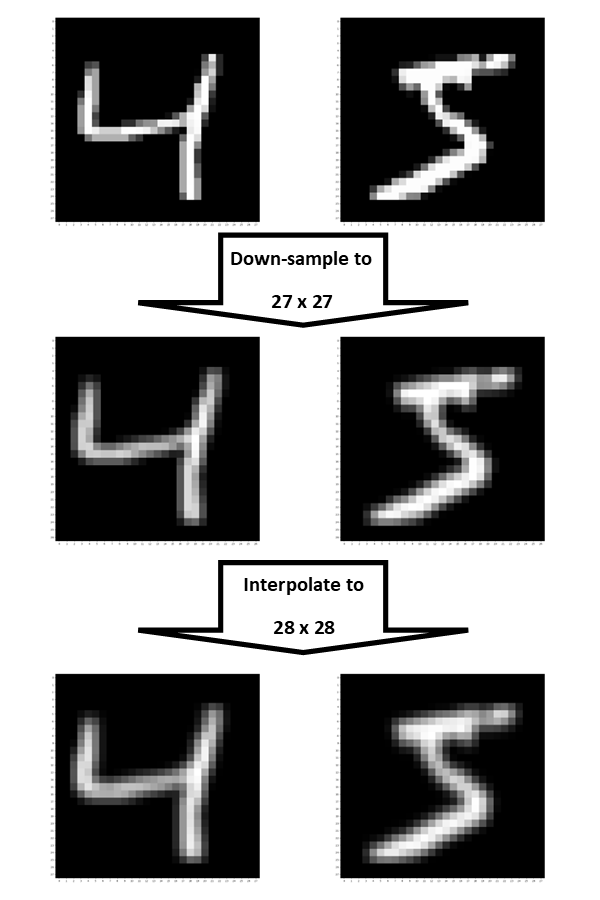
\includegraphics[scale=0.5]{fig/caseStudy1.png}
    \caption{Example image preprocessing for Case Study 1}
    \label{fig:caseStudy1}
\end{figure}

\subsection{Case Study 2}
 Each input sample is subject to a 2D average pooling filter which uses a 2 x 2 window, with a 2 x 2 step size, which brings the image from 28 x 28 down to 14 x 14. Here, images are down-sized to a total of 196 pizels or $25\%$ of the original size. This reductions is comparable to the compression ratio of PNG images, however, due to the 2D average pooling operation, exact information about the original pixel brightnesses are lost. Despite this, the contents of each image are still recognizable, but appear very pixelated.
 \begin{figure}[!h]
    \centering
    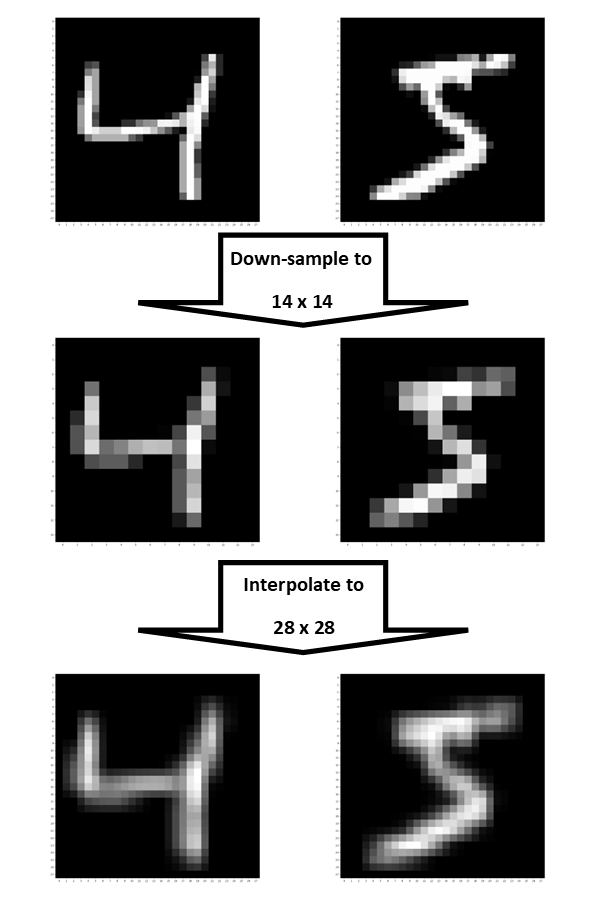
\includegraphics[scale=0.5]{fig/caseStudy2.png}
    \caption{Example image preprocessing for Case Study 2}
    \label{fig:caseStudy2}
\end{figure}

\subsection{Case Study 3}
Each input sample is subject to a 2D average pooling filter which uses a 3 x 3 window, with a 1 x 1 step size, which brings the image from 28 x 28 down to 26 x 26. In this format, each image is 676 pixels or about $86\%$ of the original size.
\begin{figure}[!h]
    \centering
    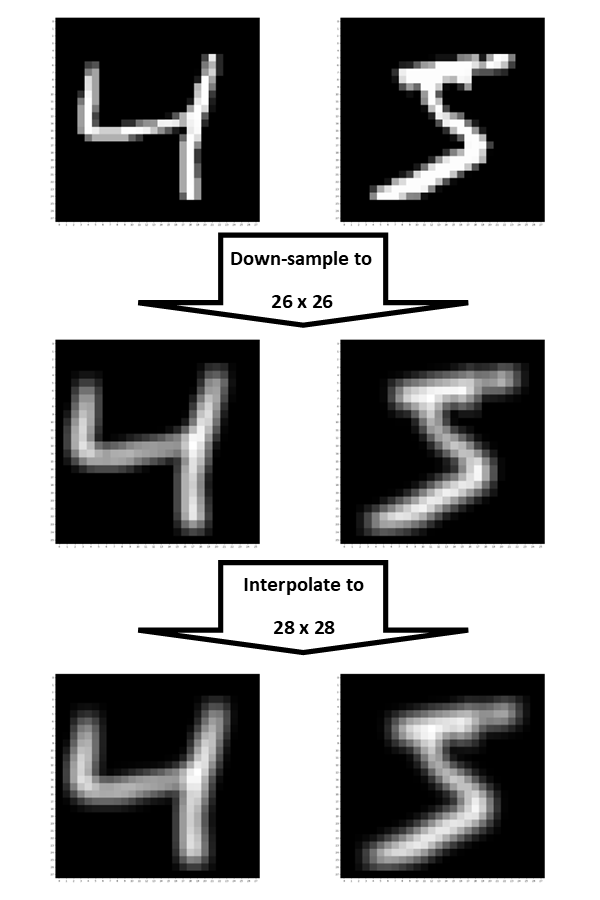
\includegraphics[scale=0.5]{fig/caseStudy3.png}
    \caption{Example image preprocessing for Case Study 3}
    \label{fig:caseStudy3}
\end{figure}

\subsection{Case Study 4}[
Each input sample is subject to a 2D average pooling filter which uses a 3 x 3 window, with a 2 x 2 step size, which brings the image from 28 x 28 down to 13 x 13. Here, images are reduced to 169 pixels, or less than $22\%$ of their original size. This is the most compressed variation in the case-studies. Just like Case Study 2, the pooling procedure generates a very pixelated version of the original image and interpolating it back up to size produces a "fuzzy-looking" varation of the original.
\begin{figure}[!h]
    \centering
    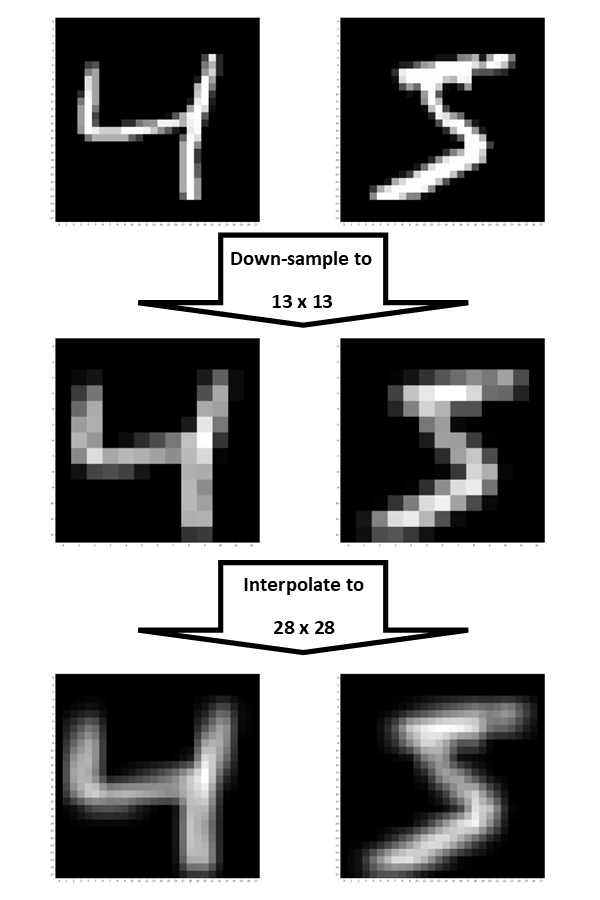
\includegraphics[scale=0.5]{fig/caseStudy4.png}
    \caption{Example image preprocessing for Case Study 4}
    \label{fig:caseStudy4}
\end{figure}

% ================================================================
\section{Experimental Results}

\textit{Data has been generated, but Need to finish plots here}

% ================================================================
\section{Conclusion}  

% ================================================================

\begin{thebibliography}{9}
\bibliographystyle{apalike}

\bibitem{Geron}
Geron, Aurelien. \textit{Hands-on Machine Learning with Scikit-Learn and TensorFlow: Concepts, Tools, and Techniques to Build Intelligent Systems}. O'Reilly, 2017.

\bibitem{Geron2}
Geron, Aurelien. \textit{Hands-on Machine Learning with Scikit-Learn and TensorFlow: Concepts, Tools, and Techniques to Build Intelligent Systems}. 2nd ed., O'Reilly, 2019.

\bibitem{Goodfellow}
Goodfellow, Ian, et al.\textit{Deep Learning}. MIT Press, 2017.

\bibitem{James}
James, Gareth, et al. \textit{An Introduction to Statistical Learning with Applications in R}. Springer, 2017.

\bibitem{Loy}
Loy, James , \textit{Neural Network Projects with Python}. Packt Publishing, 2019

\bibitem{Matplotlib}
John D. Hunter. Matplotlib: A 2D Graphics Environment, Computing in Science \& Engineering, 9, 90-95 (2007), DOI:10.1109/MCSE.2007.55

\bibitem{Numpy}
Harris, C.R., Millman, K.J., van der Walt, S.J. et al. Array programming with NumPy. Nature 585, 357–362 (2020). DOI: 0.1038/s41586-020-2649-2. 

\bibitem{Scipy}
Pauli Virtanen, et. al. SciPy 1.0: Fundamental Algorithms for Scientific Computing in Python. Nature Methods, 17(3), 261-272.

\bibitem{Sklearn}
Fabian Pedregosa, et. al. Scikit-learn: Machine Learning in Python, Journal of Machine Learning Research, 12, 2825-2830 (2011) 

\bibitem{Tensorflow}
TensorFlow: Large-scale machine learning on heterogeneous systems,
2015. Software available from tensorflow.org.

\bibitem{Virtanen}
Virtanen, Tuomas, et al. \textit{Computational Analysis of Sound Scenes and Events.} Springer, 2018.

\end{thebibliography}

% ================================================================

\end{document}
